%Este trabalho está licenciado sob a Licença Creative Commons Atribuição-CompartilhaIgual 4.0 Internacional. Para ver uma cópia desta licença, visite https://creativecommons.org/licenses/by-sa/4.0/ ou envie uma carta para Creative Commons, PO Box 1866, Mountain View, CA 94042, USA.

\chapter{Geometria}
\section{Circunferência}

\vskip0.3cm

\colorbox{azul}{
 \begin{minipage}{0.9\linewidth}
 \begin{center}
 \textbf{Circunferência}

  É o conjunto de todos os pontos do plano que estão a uma mesma distância não nula $r$ de um ponto fixo $O$. Exemplo a figura abaixo.
 \end{center}
 \end{minipage}}

 \vskip0.3cm

 \begin{center}
 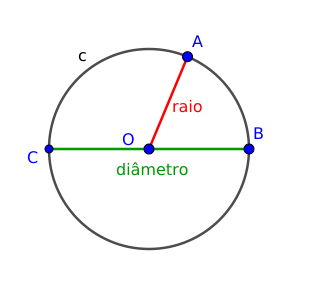
\includegraphics[width=4cm]{./cap_geometria/figs/circunferencia}
 \end{center}

Este ponto fixo $O$ é o centro da circunferência, e esta distância $r$ é o raio da circunferência, que é igual ao tamanho do segmento $\overline{OA}$, por isso este segmento é também chamado de raio da circunferência.

Os segmentos $\overline{CO}$ e $\overline{OB}$, são também raios desta circunferência. Já o segmento $\overline{CB}$ é chamado diâmetro da circunferência $d$ e sua medida é o dobro da medida do raio.

\destaque{d= 2r}

O \textbf{comprimento} ou \textbf{perímetro} da circunferência é o tamanho da medida do contorno da circunferência e é dado pela fórmula:

\destaque{C= 2 \pi r}.

Sendo $C$ o comprimento, \destaque{\pi \approx 3,14} uma constante e $r$ o raio da circunferência.

A \textbf{área} da circunferência determina o tamanho da superfície desta figura e é dada pela fórmula:

\destaque{A= \pi r^2}.


\section{Polígonos}

\vskip0.3cm

\colorbox{azul}{
 \begin{minipage}{0.9\linewidth}
 \begin{center}
 \textbf{Polígonos}

  São figuras geométricas fechadas, formadas por segmentos de reta.

  Estas figuras são caracterizadas pelos seguintes elementos: ângulos, vértices, diagonais e lados.
 \end{center}
 \end{minipage}}

 \vskip0.3cm

  Os polígonos recebem nomes especiais de acordo com o número de lados que possuem. Veja na tabela abaixo o nome de alguns polígonos.

   %\vskip0.3cm

 \begin{table}[H]
 \centering
 \begin{tabular}{|c|c|c|c|} \hline
 \rowcolor{cinza}
 Nome do polígono & Nº de Vértices & Nº de Lados & Polígonos  \\ \hline
 Triângulo & 3 & 3 & 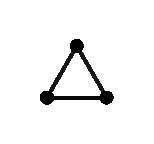
\includegraphics[width=2cm]{./cap_geometria/figs/pol3} \\ \hline
 Quadrilátero & 4 & 4 & 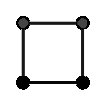
\includegraphics[width=2cm]{./cap_geometria/figs/pol4} \\ \hline
 Pentágono & 5 & 5 & 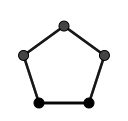
\includegraphics[width=2cm]{./cap_geometria/figs/pol5} \\ \hline
 Hexágono & 6 & 6 & 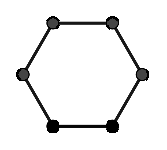
\includegraphics[width=2cm]{./cap_geometria/figs/pol6} \\ \hline
 Heptágono & 7 & 7 & 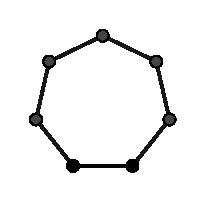
\includegraphics[width=2cm]{./cap_geometria/figs/pol7} \\ \hline
 Octógono & 8 & 8 & 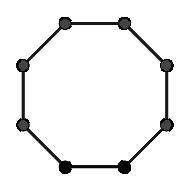
\includegraphics[width=2cm]{./cap_geometria/figs/pol8} \\ \hline
 Eneágono & 9 & 9 & 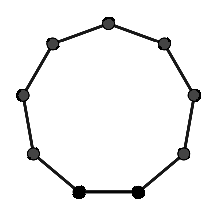
\includegraphics[width=2cm]{./cap_geometria/figs/pol9} \\ \hline
 Decágono & 10 & 10 & 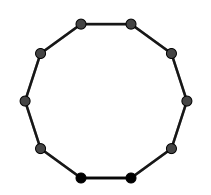
\includegraphics[width=3cm]{./cap_geometria/figs/pol10} \\ \hline
 \end{tabular}
\end{table}

 \begin{table}[H]
 \centering
 \begin{tabular}{|c|c|c|c|} \hline
 \rowcolor{cinza}
 Nome do polígono & Nº de Vértices & Nº de Lados & Polígonos  \\ \hline
 Undecágono & 11 & 11 & 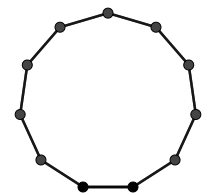
\includegraphics[width=3cm]{./cap_geometria/figs/pol11} \\ \hline
 Dodecágono & 12 & 12 & 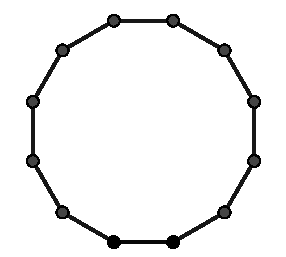
\includegraphics[width=3cm]{./cap_geometria/figs/pol12} \\ \hline
 Pentadecágono & 15 & 15 & 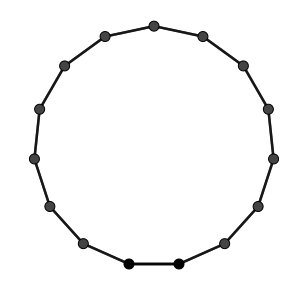
\includegraphics[width=3cm]{./cap_geometria/figs/pol15} \\ \hline
 Icoságono & 20 & 20 & 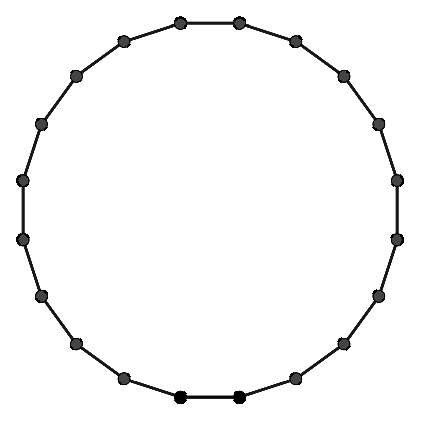
\includegraphics[width=3cm]{./cap_geometria/figs/pol20} \\ \hline
 \end{tabular}
\end{table}

\subsection{Classificação dos Quadriláteros}

De acordo com a tabela acima um quadrilátero é um polígono que possui 4 lados.

Por sua importância na Geometria, alguns quadriláteros têm denominação própria. Os principais quadriláteros são os seguintes:

\textbf{Trapézio}

É um quadrilátero que tem dois lados paralelos.

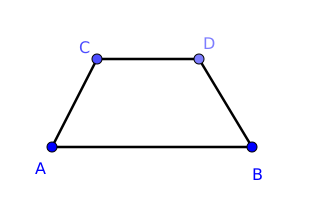
\includegraphics[width=4cm]{./cap_geometria/figs/trapezio}


\textbf{Paralelogramo}

É um quadrilátero que tem dois pares de lados paralelos.

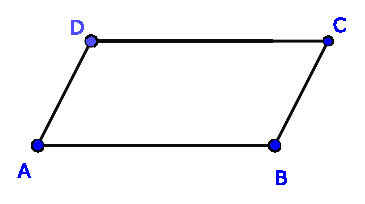
\includegraphics[width=4cm]{./cap_geometria/figs/paralelogramo}

\newpage
\textbf{Retângulo}

É um paralelogramo que tem todos os ângulos retos (iguais a $90\degree$).

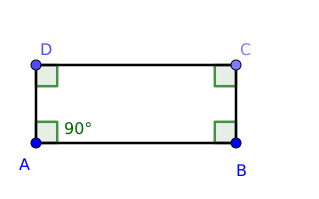
\includegraphics[width=4cm]{./cap_geometria/figs/retangulo}


\textbf{Losango}

É um paralelogramo em que todos os lados têm a mesma medida. Vale observar também que as diagonais do losango se encontram em seus pontos médios formando ângulo de $90\degree$.

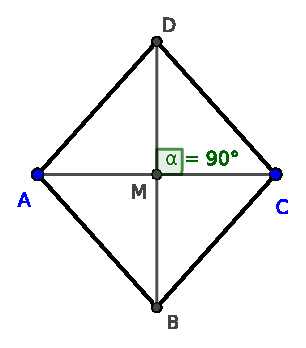
\includegraphics[width=4cm]{./cap_geometria/figs/losango}


\textbf{Quadrado}

É um paralelogramo em que todos os lados têm medidas iguais e todos os ângulos são retos.

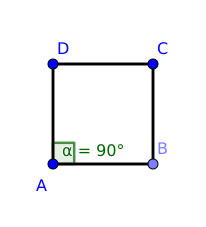
\includegraphics[width=4cm]{./cap_geometria/figs/quadrado}


\subsection{Classificação dos Triângulos}

Como visto anteriormente um triângulo é um polígono que possui 3 lados. É importante saber que a soma dos ângulos internos de qualquer triângulo mede $180\degree$.

Os triângulos são classificados de acordo com o tamanho de seus lados, e também de acordo com as medidas de seus ângulos internos. Esta classificação é apresentada nas tabelas abaixo.

\begin{table}[H]
\centering
 \begin{tabular}{|c|c|c|} \hline
 \rowcolor{cinza}
 \multicolumn{3}{|c|}{\textbf{Quanto aos lados}} \\ \hline
  Equilátero & Possui os três lados iguais & 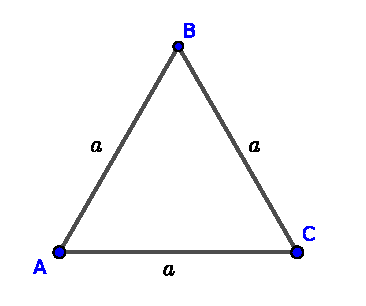
\includegraphics[width=3cm]{./cap_geometria/figs/triangulo_equi} \\ \cline{1-3}
                   Isósceles & Possui dois lados iguais & 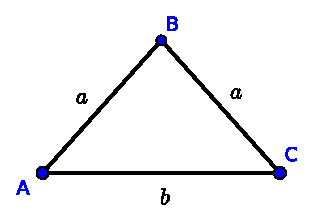
\includegraphics[width=3cm]{./cap_geometria/figs/triangulo_isos}\\ \cline{1-3}
                   Escaleno & Possui os três lados diferentes & 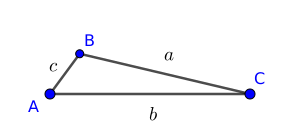
\includegraphics[width=3cm]{./cap_geometria/figs/triangulo_esc} \\ \hline
\end{tabular}
\end{table}

Vale aqui ressaltar mais algumas propriedades destes triângulos:
\begin{itemize}
 \item Em um \textbf{triângulo equilátero} todos os ângulos internos medem $60\degree$;
 \item Em um \textbf{triângulo isósceles} os ângulos da base (lado de medida diferente), possuem a mesma medida.
\end{itemize}


\begin{table}[H]
\centering
 \begin{tabular}{|c|c|c|} \hline
 \rowcolor{cinza}
 \multicolumn{3}{|c|}{\textbf{Quanto aos ângulos}} \\ \hline
 Obtusângulo & Possui um ângulo medindo mais que $90\degree$ & 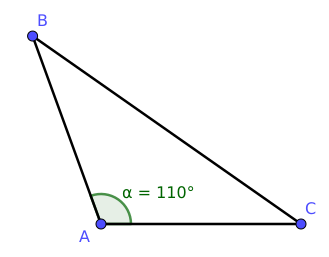
\includegraphics[width=3cm]{./cap_geometria/figs/triangulo_obt} \\ \cline{1-3}
   Retângulo & Possui um ângulo reto, que mede $90\degree$ & 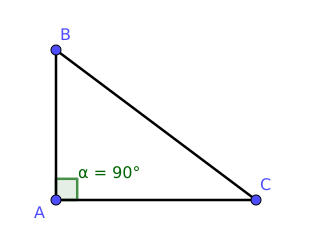
\includegraphics[width=3cm]{./cap_geometria/figs/triangulo_ret}
    \\ \cline{1-3}
   Acutângulo & Possui todos os ângulos medindo menos que $90\degree$ & 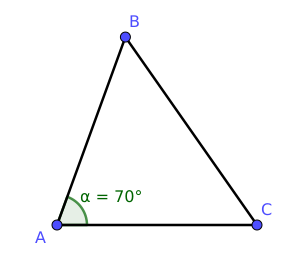
\includegraphics[width=3cm]{./cap_geometria/figs/triangulo_acu} \\ \hline
 \end{tabular}
\end{table}

Vale neste momento observar que o \textbf{triângulo retângulo} é o triângulo que satisfaz o teorema de Pitágoras, e também é o triângulo usado na trigonometria.


\subsection{Perímetro}

\vskip0.3cm
 \colorbox{amarelo}{
 \begin{minipage}{0.9\linewidth}
 \begin{center}
  O \textbf{perímetro} de um polígono qualquer é dado pela soma das medidas de seus lados.
 \end{center}
 \end{minipage}}
 \vskip0.3cm


Dada uma região com uma forma poligonal, é o perímetro do polígono que nos diz por exemplo, quantos metros de cerca precisamos comprar para cercar esta região.

\subsection{Área}

A área de uma região poligonal nos diz por exemplo de quantas lajotas precisamos para cobrir a região. Mas calcular a área é um pouco mais complicado, por que o cálculo da área depende do polígono que estamos considerando, vou listas aqui somente as mais usadas.

\textbf{Triângulo:}
\begin{multicols}{2}

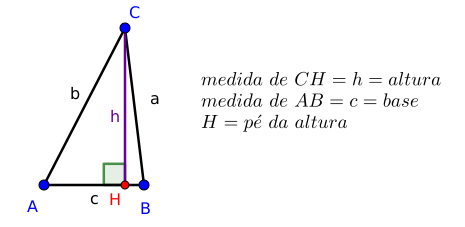
\includegraphics[width=7cm]{./cap_geometria/figs/triangulo} \\
A área de um triângulo é dada pela fórmula

\destaque{A= \frac{b \cdot h}{2}}

na qual $b$ representa a base do triângulo e $h$ a altura.
\end{multicols}

\textbf{Quadrado}
\begin{multicols}{2}
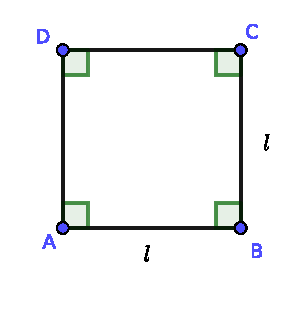
\includegraphics[width=3cm]{./cap_geometria/figs/quadrado_L} \\
A área do quadrado é dada pela fórmula

\destaque{A= l \cdot l= l^2}

onde $l$ representa o lado do quadrado.
\end{multicols}

\textbf{Retângulo}
\begin{multicols}{2}
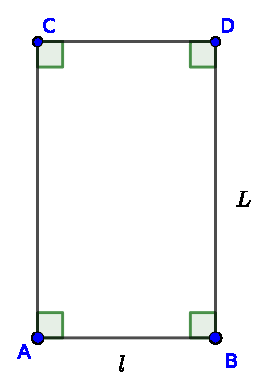
\includegraphics[width=3cm]{./cap_geometria/figs/retangulo_L} \\
A área do retângulo é dada pela fórmula

\destaque{A= L \cdot l}

onde $L$ representa o lado maior e $l$ representa o lado menor.
\end{multicols}

\textbf{Paralelogramo}
\begin{multicols}{2}
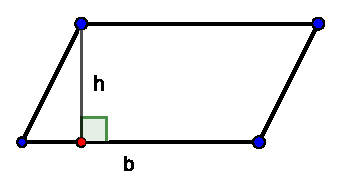
\includegraphics[width=5cm]{./cap_geometria/figs/paralelogramoL} \\
A área do paralelogramo é dada pela fórmula

\destaque{A= b \cdot h}

onde $b$ representa a base e $h$ representa a altura.
\end{multicols}

\newpage

\textbf{Losango}
\begin{multicols}{2}
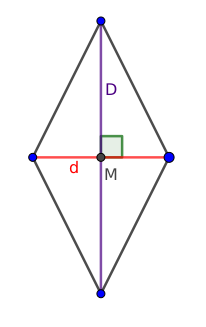
\includegraphics[width=3cm]{./cap_geometria/figs/losangoL} \\
A área do losango é dada pela fórmula

\destaque{A= \frac{D \cdot d}{2}}

onde $D$ representa a diagonal maior e $d$ representa a diagonal menor.
\end{multicols}

\textbf{Trapézio}
\begin{multicols}{2}
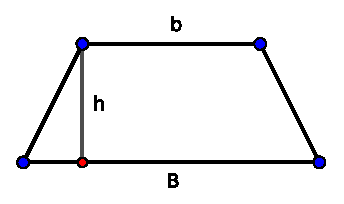
\includegraphics[width=5cm]{./cap_geometria/figs/trapezioL} \\
A área do trapézio é dada pela fórmula

\destaque{A= \frac{(B+b)\cdot h}{2}}

onde $B$ representa a base maior, $b$ a base menor e $h$ a altura do trapézio.
\end{multicols}

\section{Sólidos}

\vskip0.3cm

\colorbox{azul}{
 \begin{minipage}{0.9\linewidth}
 \begin{center}
 \textbf{Sólidos}

  Sólidos geométricos são os objetos tridimensionais definidos no espaço.

  O conjunto de todos os sólidos geométricos está dividido em três grupos: poliedros, corpos redondos, e outros.

 \end{center}
 \end{minipage}}

 \vskip0.3cm

 Alguns exemplos de sólidos geométricos são: cubos, pirâmides, prismas, cilindros, cones e esferas.



\begin{figure}[H]
\center
\subfigure[ref1][]{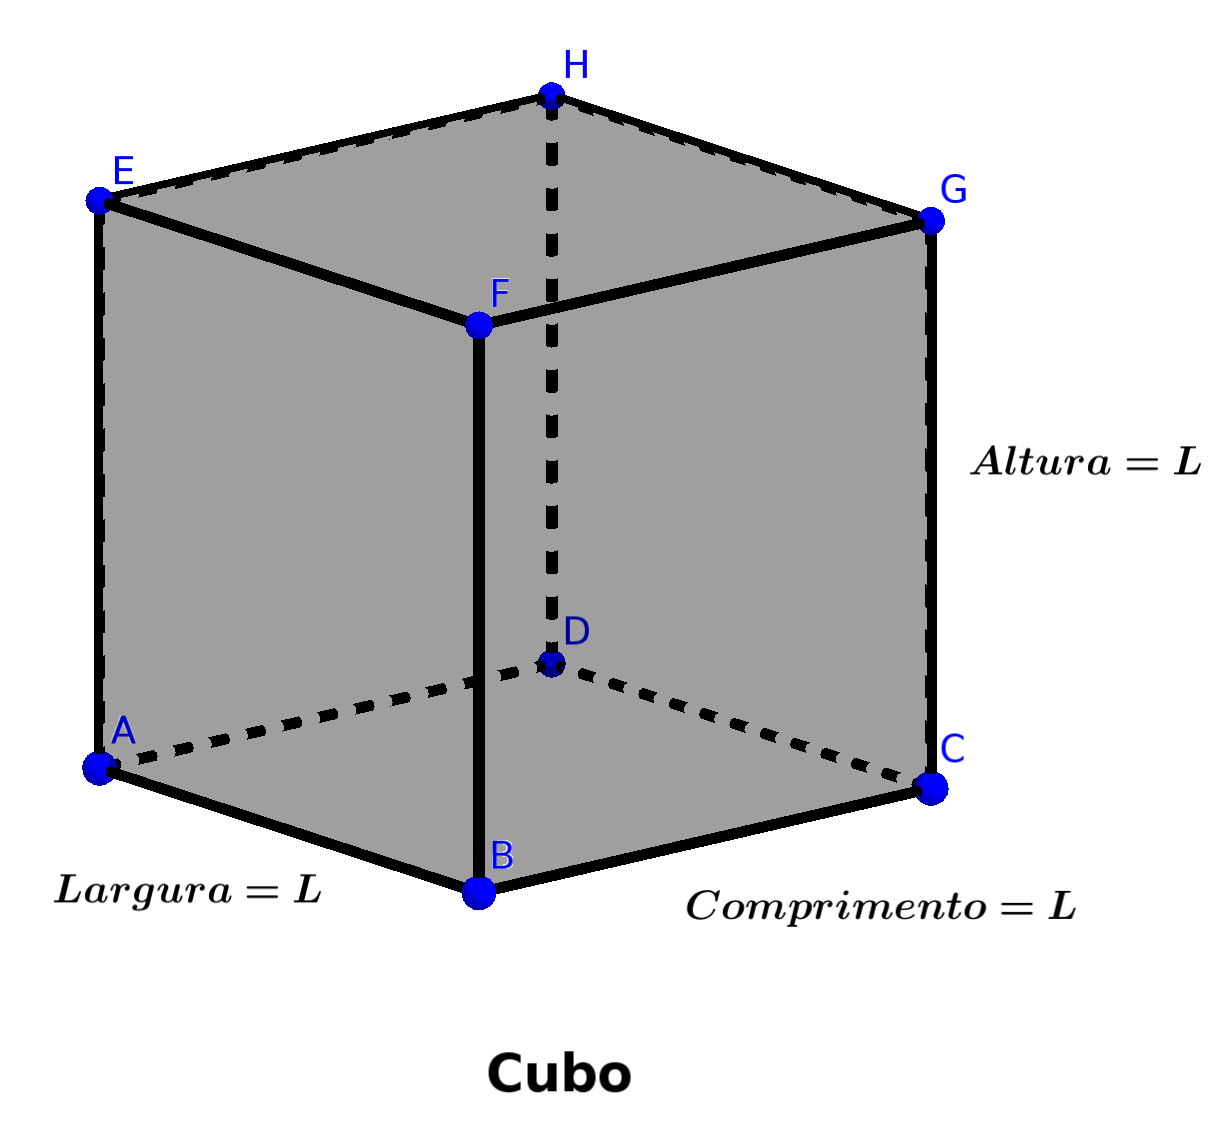
\includegraphics[width=6cm]{./cap_geometria/figs/cubo}}
\qquad
\subfigure[ref2][]{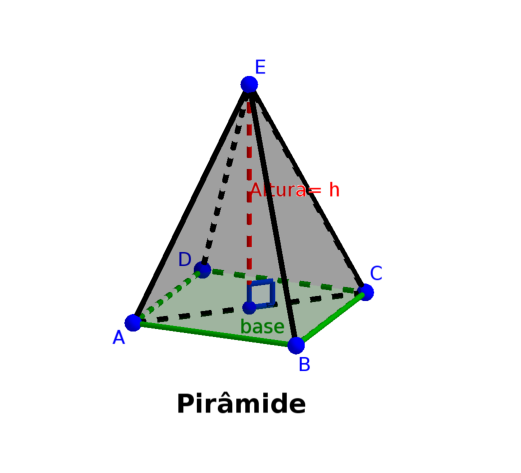
\includegraphics[width=6cm]{./cap_geometria/figs/piramide_quadrada}}
\end{figure}

\begin{figure}[H]
\center
\subfigure[ref2][]{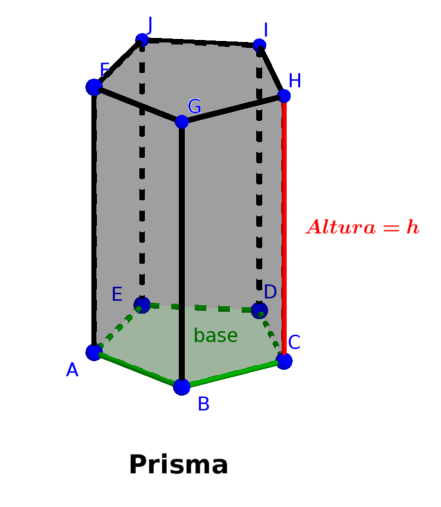
\includegraphics[width=6cm]{./cap_geometria/figs/prisma_pentagono}}
\qquad
\subfigure[ref2][]{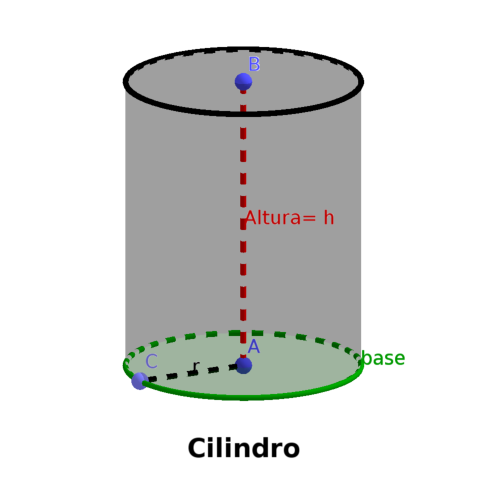
\includegraphics[width=6cm]{./cap_geometria/figs/cilindro}}
\qquad
\subfigure[ref2][]{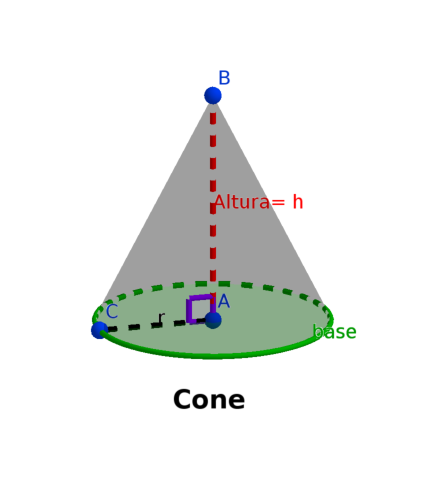
\includegraphics[width=6cm]{./cap_geometria/figs/cone}}
\qquad
\subfigure[ref2][]{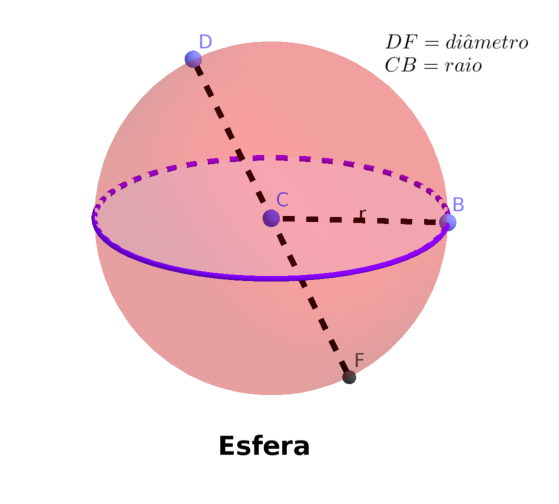
\includegraphics[width=6cm]{./cap_geometria/figs/esfera}}

\end{figure}


 \textbf{Poliedros}

 São sólidos geométricos limitados por faces, que, por sua vez, são polígonos. Assim, qualquer sólido geométrico cuja superfície seja formada somente por polígonos é um poliedro. As linhas formadas pelo encontro entre duas faces de um poliedro é chamada de aresta e qualquer ponto de encontro entre arestas é chamado de vértice.

O grupo dos poliedros é dividido em outros três grupos: cubos, pirâmide, prismas, e outros.

\textbf{Corpos redondos}

São aqueles sólidos que possuem curvas em vez de alguma face e que, se colocados sobre uma superfície plana levemente inclinada, rolam.

São exemplos de corpos redondos: cilindros, cones e esferas.

 \newpage
\subsection{Volume}

\begin{multicols}{2}
 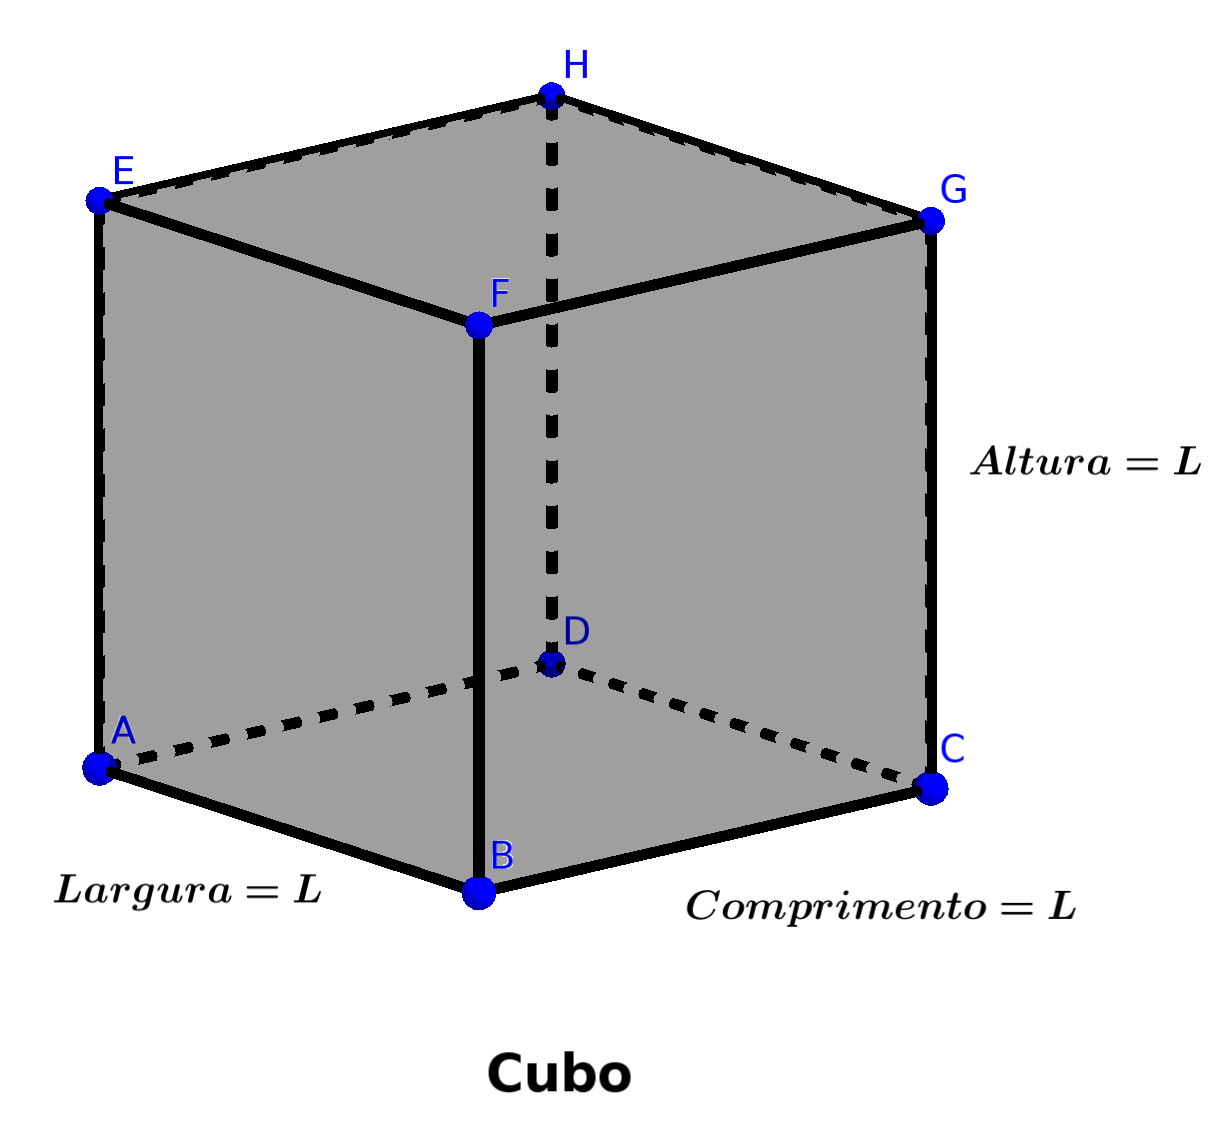
\includegraphics[width=5cm]{./cap_geometria/figs/cubo} \\

 O volume do cubo é dado pela equação:
 
 \destaque{V= L \cdot L \cdot L= L^3}
 
 Onde $L$ é a medida do lado do cubo.
\end{multicols}

\begin{multicols}{2}
 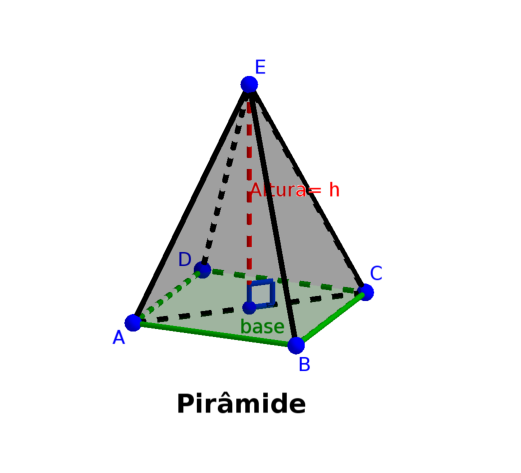
\includegraphics[width=6cm]{./cap_geometria/figs/piramide_quadrada} \\
 O volume da pirâmide é dado pela equação:
 
 \destaque{V= \frac{1}{3} \cdot A_b \cdot h }
 
 Onde $A_b$ é a área da base da pirâmide que varia de acordo com o polígono que está na base, e $h$ é a altura da pirâmide.
\end{multicols}

\begin{multicols}{2}
 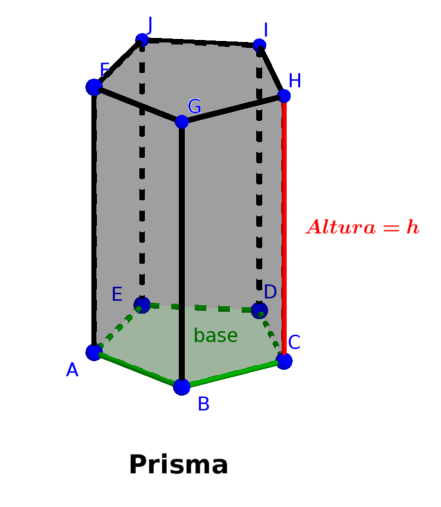
\includegraphics[width=6cm]{./cap_geometria/figs/prisma_pentagono} \\
 O volume do prisma é dado pela equação:
 
 \destaque{V= A_b \cdot h }

 Onde $A_b$ é a área da base do prisma que varia de acordo com o polígono que está na base, e $h$ é a altura do prisma.

 Um caso particular de prisma é o \textbf{paralelepípedo} que é um prisma cuja base é um quadrado ou um retângulo.
\end{multicols}

\begin{multicols}{2}
 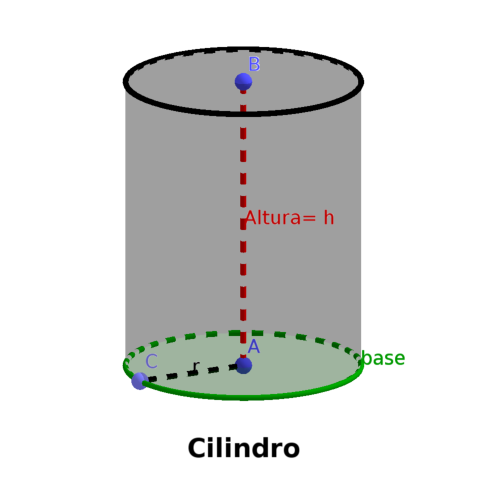
\includegraphics[width=6cm]{./cap_geometria/figs/cilindro} \\
 O volume do cilindro é dado pela equação:
 
 \destaque{V= A_b \cdot h= \pi \cdot r^2 \cdot h }

 Onde $A_b$ é a área da base do cilindro que é uma circunferência, e $h$ é a altura do cilindro.
\end{multicols}

\begin{multicols}{2}
 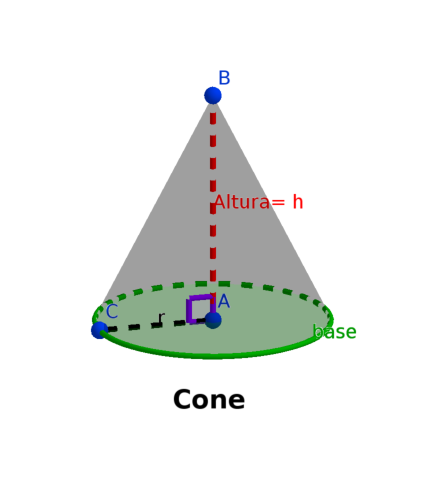
\includegraphics[width=6cm]{./cap_geometria/figs/cone} \\

 O volume do cone é dado pela equação:
 
 \destaque{V= \frac{1}{3} \cdot A_b \cdot h= \frac{1}{3} \cdot \pi \cdot r^2 \cdot h = \frac{\pi \cdot r^2 \cdot h}{3}}

 Onde $A_b$ é a área da base do cone que é uma circunferência, e $h$ é a altura do cone.
\end{multicols}

\begin{multicols}{2}
 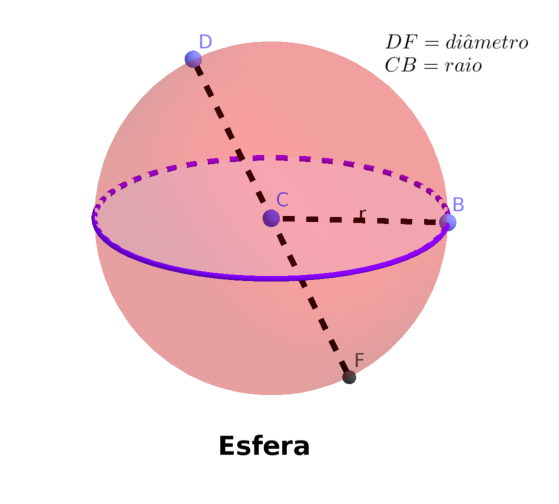
\includegraphics[width=6cm]{./cap_geometria/figs/esfera} \\

 O volume da esfera é dado pela equação:
 
 \destaque{V= \frac{4}{3} \cdot \pi \cdot r^3= \frac{4 \cdot \pi \cdot r^3}{3}}
 
 Onde $r$ é o raio da esfera, e $\pi \approx 3,14$ é uma constante.
\end{multicols}
